\documentclass[serif]{beamer}
%\usefonttheme[onlymath]{serif}
\usepackage{amsmath}
\usepackage{url}
\usepackage{ucs}
\usepackage[utf8x]{inputenc}
\usepackage[ngerman]{babel}
\usepackage{color}
\usepackage{media9}
\usepackage{hyperref}
\usepackage{bookman}

\usetheme{Boadilla}
\setbeamertemplate{footline}

\usecolortheme{lily}
\usefonttheme{serif}
\useinnertheme{circles}
\setbeamercovered{transparent}
\beamertemplatenavigationsymbolsempty

\definecolor{darkgreen}{rgb}{0,0.5,0}

\hypersetup{
    bookmarks=true,
    unicode=true,
    pdftoolbar=true,
    pdfmenubar=true,
    pdffitwindow=false,
    pdfstartview={FitH},
    pdftitle={Stabilität invertierter Pendel},
    pdfauthor={Michael Hartmann},
    pdfsubject={Vortrag über Stabilität invertierter Pendel},
    pdfcreator={vim},
    pdfproducer={pdflatex},
    pdfkeywords={Mathieu} {Stabilität} {invertierte Pendel},
    pdfnewwindow=true,
    colorlinks=true,
    linkcolor=black,
    citecolor=green,
    filecolor=magenta,
    urlcolor=darkgreen
}



\title{Stabilität invertierter Pendel}
\institute{Kaffeeseminar}
\author{Michael Hartmann}
\date{4. November 2016}


\titlegraphic{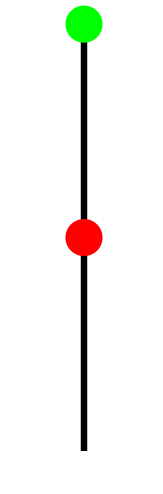
\includegraphics[scale=0.3]{images/title.png}}


\begin{document}

\begin{frame}
    \titlepage
\end{frame}


\frame{
    \frametitle{Überblick}
    \tableofcontents 
}

\section{Was ist ein Doppelpendel?}

\frame {
    \frametitle{Was ist ein Doppelpendel?}

    \begin{minipage}[b]{0.35\textwidth} 
    \begin{center}
    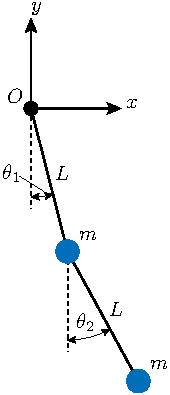
\includegraphics[scale=1.1]{images/sketch.pdf}
    \end{center}
    \end{minipage}
    \hfill
    \begin{minipage}[b]{0.6\textwidth}
	Koordinaten
    \begin{align}
    \nonumber
    x_1 &= L \sin\theta_1 \\
    \nonumber
    y_1 &= -L \cos\theta_1 \\
    \nonumber
    x_2 &= L \sin\theta_1 + L \sin\theta_2 \\
    \nonumber
    y_2 &= -L \cos\theta_1 - L \cos\theta_2
    \end{align}

    \vfill

    Lagrange-Funktion
    \begin{align}
    \nonumber
    \mathcal{L} &= T-V \\
    \nonumber
    T &= \frac{1}{2} m v^2 \\
    \nonumber
    V &= mgL \left( 3-2\cos\theta_1-\cos\theta_2\right)
    \end{align}
    \end{minipage}
}

\frame {
    \frametitle{Linearisieren um $\theta_1\approx\theta_2\approx\pi$}

    \only<1>
    {
    Kinetische Energie
    \begin{equation}
    \nonumber
    T = \frac{1}{2} m \left( \dot x_1^2 + \dot y_1^2 + \dot x_2^2 + \dot y_2^2\right)
    \approx \frac{1}{2} mL^2 \left( 2\dot\theta_1^2  + \dot\theta_2^2 + \dot\theta_1\dot\theta_2\right)
    \end{equation}

    \vfill

    Potentielle Energie ($\Delta_j \equiv \theta_j-\pi$)
    \begin{equation}
    \nonumber
    V = mgL\left(3-2\cos\theta_1-\cos\theta_2\right) = mgL\left(6-\Delta_1^2-\frac{\Delta_2^2}{2}\right)
    \end{equation}

    \vfill

    Lagrange-Funktion
    \begin{equation}
    \nonumber
    \mathcal{L} \approx \frac{1}{2} mL^2 \left( 2\dot \Delta_1^2  + \dot \Delta_2^2 + \dot \Delta_1\dot \Delta_2\right) + mgL\left( \Delta_1^2 + \frac{\Delta_2^2}{2} -6\right)
    \end{equation}
    }

    \only<2>
    {
    \vfill

    Euler-Lagrange-Gleichungen
    \begin{equation}
    \nonumber
    \frac{\mathrm{d}}{\mathrm{d}t} \frac{\partial\mathcal{L}}{\partial\dot \Delta_j} - \frac{\partial\mathcal{L}}{\partial \Delta_j} = 0
    \end{equation}

    Bewegungsgleichungen
    \begin{equation}
    \nonumber
    \frac{L}{2g}
    \begin{pmatrix}
    2 & 1 \\
    2 & 2
    \end{pmatrix}
    \begin{pmatrix}
    \ddot \Delta_1 \\ \ddot \Delta_2
    \end{pmatrix}
    =
    \begin{pmatrix}
    \Delta_1 \\ \Delta_2
    \end{pmatrix}
    \end{equation}

    \vfill

    Eigenfrequenzen
    \begin{equation}
    \nonumber
    \omega_1 = \sqrt{\frac{g}{L}} \sqrt\frac{2}{2+\sqrt{2}}, \qquad
    \omega_2 = \sqrt{\frac{g}{L}} \sqrt\frac{2}{2-\sqrt{2}}
    \end{equation}
    }
}

\frame {
    \frametitle{Normalkoordinaten}

    \only<1>
    {
    Kleine Abweichungen $\Delta\approx0$ in Normalkoordinaten
    \begin{equation}
    \nonumber
    \ddot X_j - \omega_j^2 X_j = 0, \qquad j=1,\dots,N
    \end{equation}

    \vfill

    Aufhängung $O$ oszilliere nun mit Frequenz $\omega_0$ und Amplitude $\epsilon$
    \begin{equation}
    \nonumber
    \ddot X_j - \omega_j^2 \left( 1+\frac{\epsilon \omega_0^2}{g}\cos{(\omega_0 t)} \right)X_j = 0 \qquad j=1,\dots,N
    \end{equation}

    \vfill
    }

    Reskalieren mit $\tau = \omega_0 t$
    \begin{equation}
    \nonumber
    \frac{\mathrm{d}^2 X_j}{\mathrm{d}\tau^2} + \left( \alpha_j+\beta_j\cos\tau \right) X_j = 0, \qquad j=1,\dots,N
    \end{equation}
    \begin{equation}
    \nonumber
    \text{mit} \qquad \alpha_j = - \omega_j^2/\omega_0^2, \quad \beta_j = -\omega_j^2\epsilon/g
    \end{equation}

    \only<2>
    {
    \vfill
    \begin{center}
    $\Rightarrow$ $N$ ungekoppelte \hyperlink{https://en.wikipedia.org/wiki/Mathieu_function}{Mathieu Gleichungen}
    \end{center}
    }

}

\frame {
    \frametitle{Indischer Seiltrick}

    \begin{center}
    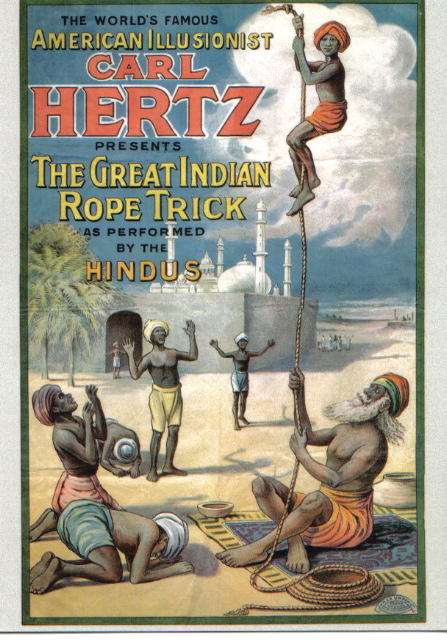
\includegraphics[scale=0.3]{images/Indian-Rope-Trick.jpg} \quad
    \includegraphics[scale=0.618]{images/Indian-Rope-Trick_2.jpg}
    \end{center}

    \vfill

    \hrule
    {
    \tiny
    \begin{flushright}
    Quelle: \url{https://en.wikipedia.org/wiki/Indian_rope_trick}
    \end{flushright}
    }
}

\frame {
    \frametitle{Quellennachweis}

    Bibliographie
    \begin{itemize}
    \item \hyperlink{http://dx.doi.org/10.1098/rspa.1993.0142}{D. J. Acheson, \textbf{A pendulum theorem}, The Royal Society (1993)}
    \end{itemize}
}

\end{document}
